\documentclass[a4paper]{article}

\usepackage[
    a4paper,
    left=0.4in,
    right=0.4in,
    top=0.1in,
    bottom=0.1in
]{geometry}
\usepackage{url,parskip} 	%other packages for formatting
\usepackage[usenames,dvipsnames]{xcolor}
\usepackage{titlesec}					%custom \section
\usepackage{hyperref}
\usepackage{stix}
\usepackage[absolute]{textpos}
\usepackage{fontspec}
\usepackage{graphicx}
\usepackage{color}
\usepackage{lipsum}
\usepackage{ragged2e}
\usepackage{fontspec}
\usepackage{fontawesome5}
\usepackage{pgffor} % Standard package for looping

\hypersetup{colorlinks,breaklinks,urlcolor=linkcolour, linkcolor=linkcolour}
\defaultfontfeatures{Mapping=tex-text}
\titleformat{\section}{\large\scshape\raggedright}{}{0em}{}
\titlespacing{\section}{0pt}{3pt}{3pt}
\hyphenation{im-pre-se}
\textblockorigin{2mm}{0.65\paperheight}

\setlength{\TPHorizModule}{30mm}
\setlength{\TPVertModule}{\TPHorizModule}
\setlength{\parindent}{0pt}

\definecolor{linkcolour}{rgb}{0,0.2,0.6}
\definecolor{previousCompany}{rgb}{0.1,0.1,0.1}
\definecolor{previousRole}{rgb}{0.2,0.2,0.2}
\definecolor{previousWork}{rgb}{0.2,0.2,0.2}
\definecolor{currentCompany}{rgb}{0.1,0.1,0.1}
\definecolor{currentRole}{rgb}{0.1,0.1,0.1}
\definecolor{currentWork}{rgb}{0.1,0.1,0.1}
\newcommand{\apple}{\char"F8FF}
\newcommand{\SectionSize}{\large}
\newcommand{\SpaceBetweenJobs}{\vspace{-1em}}
\newcommand{\nyu}{\raisebox{-0.8ex}{\includegraphics[height=1.2em]{NYU.png}}}
\newcommand{\CurrentWorkBullet}[1]{
  \noindent\hspace*{2.0em}\textbullet & {\fontspec{Inter} #1} \\
}
\newcommand{\PreviousWorkBullet}[1]{
  \noindent\hspace*{2.0em}$\circ$ & {\fontspec{Inter} #1} \\
}
\usepackage{xcolor} % Required to change text and icon colors

\usepackage{tikz}

\newcommand*{\partcirc}[2]{%
	\hspace{-1em}%
	\begin{tikzpicture}[baseline=-0.6ex]
		\draw[previousWork] (0,0) circle (1ex);
		\fill[previousWork] (0,0) -- (#1:1ex) arc (#1:#2:1ex) -- cycle;
	\end{tikzpicture}%
	\hspace{1em}%
}

\newcommand*{\partcircfill}[1]{%
	\hspace{-1em}%
	\pgfmathsetmacro{\endangle}{90 - 3.6*#1}
	\begin{tikzpicture}[baseline=-0.6ex]
		\draw[previousWork] (0,0) circle (1ex);
		\fill[previousWork] (0,0) -- (90:1ex) arc (90:\endangle:1ex) -- cycle;
	\end{tikzpicture}%
	\hspace{1em}%
}

\newcommand*{\pacman}[1]{%
	\hspace{-1em}%
	\pgfmathsetmacro{\mouth}{(100-#1)*1.8}
	\begin{tikzpicture}[baseline=-0.6ex]
		\fill[previousWork] (0,0) circle (1ex);
		\fill[white] (0,0) -- (\mouth:1ex) arc (\mouth:-\mouth:1ex) -- cycle;
		\draw[previousWork] (0,0) circle (1ex);
	\end{tikzpicture}%
	\hspace{1em}%
}


\newcommand{\stars}[1]{%
    \begin{minipage}[b]{6em}% Adjust width to fit nicely inline
    \foreach \i in {1,...,5} {%
        \pgfmathparse{#1 - \i + 1}%
        \let\r=\pgfmathresult%
        \pgfmathparse{\r >= 1 ? 1 : (\r <= 0 ? 0 : 0.5)}%
        \let\status=\pgfmathresult%
        \ifdim\status pt=1pt%
            \textcolor{black!60}{\faStar}% Full star (60% black/dark grey)
        \else\ifdim\status pt=0.5pt%
            \textcolor{black!60}{\faStarHalf*}% Half star (60% black/dark grey)
        \else%
            \textcolor{black!20}{\faStar[regular]}% Empty star (Light grey outline)
        \fi\fi%
    }%
    \end{minipage}%
}


\begin{document}
\pagestyle{empty} 						% non-numbered pages
\font\fb=''[cmr10]'' 						%for use with \LaTeX command




\iffalse
comments
\fi

%\begin{comment}
%\end{comment}

%Section: Title--------------------------------------
\centering
\href{https://sap586.github.io/Resume/}{$ \Uparrow$}{Sagar Panchal}	\\
\small \href{mailto:sap586@nyu.edu}{sap586@nyu.edu}		\textbullet{+1 (607) 314-0114}		\textbullet {Broome, NY - 13901}	\\

\vspace{-0.8em}

\begin{tikzpicture}[overlay,remember picture]
\draw[gray, line width=0.8pt, rounded corners=4pt]
(-10cm,0.5cm) -- (-6cm,0.5cm) -- (-6cm,0.25cm);
\draw[gray, line width=0.8pt, rounded corners=4pt]
(-6cm,0.25cm) -- (-6cm,0cm) -- (10cm,0cm);
\draw[gray, line width=0.8pt, rounded corners=4pt]
(10cm,-1.75cm) -- (-10cm,-1.75cm);
\draw[gray, line width=0.8pt, rounded corners=4pt]
(-10cm,-3.55cm) -- (10cm,-3.55cm);
\draw[gray, line width=0.8pt, rounded corners=4pt]
(10cm,-7.1cm) -- (-4.3cm,-7.1cm) -- (-4.3cm,-6.8cm);
\draw[gray, line width=0.8pt, rounded corners=4pt]
(-4.3cm,-6.8cm) -- (-4.3cm,-6.6cm) -- (-6.3cm,-6.6cm);
\draw[gray, line width=0.8pt, rounded corners=4pt]
(-6.3cm,-6.6cm) -- (-10cm,-6.6cm);
\draw[gray, line width=0.8pt, rounded corners=4pt]
(-10cm,-27.8cm) -- (10cm,-27.8cm);

\end{tikzpicture}

%Section: About--------------------------------------
\vspace{-2.5em} % adjust value until it looks balanced
\parbox{1\linewidth}{
\section{\SectionSize{\textbf{About:}}}
\begin{justify}
{\fontspec{Inter}
{\color{currentWork}
% ABOUT_START
Software Engineer with hands-on Machine operation experience. My career has given me opportunity to work across the full technology stack, all the way from hard core mechanical installations to studying, developing and maintaining critical components of multi-million line codebases powering advanced automation systems. Currently seeking opportunities to build impactful technologies while continuing to grow as an engineer and problem solver.
% ABOUT_END
}
}
\end{justify}
}
%Section: Education--------------------------------------
\section{\SectionSize{\textbf{Education:}}}
\vspace{-2em}
\begin{tabular}{rl}
\textsc{	MS, Computer engineering \small {(3.41/4)}		}						&	--	\textsc{	Dec-17 	\faGraduationCap		}	\\
\textsc{	\large {New York University} \nyu\;		}								&	\\
\textsc{	BE, Instrumentation \& Controls Engineering \small {(7.04/10)}		}	&	--	\textsc{	Jun-14 	\faGraduationCap		}	\\
\textsc{	Gujarat Technological University	}									&	\\
\end{tabular}

%Section: Skills--------------------------------------
\section{\SectionSize{\textbf{Skills:}}}
\vspace{-2em}

\hspace{6em}\begin{tabular}{rl}	\small{}
\small{}	   {		Process Control :		}	&	{	\partcircfill{82}		Control logic implementation, execution and testing							}		\\
\small{}	   {								}	&	{	\partcircfill{78}		Process improvement and enhancement											}		\\
\small{} 	   {		Software :				}	& 	{ 	\partcircfill{70} 	Desktop - Java (Primary), C\#, Python (AI-driven workflows), Web - HTML, CSS, JS	} 		\\
\small{} 											& 	{ 	\partcircfill{80} 	Maintain large-scale \& legacy software systems 										} 		\\
\small{} 											& 	{ 	\partcircfill{85} 	Git(SourceTree, Bash) 														} 		\\
\small{}	   {		Automation :			}	&	{	\partcircfill{80}		PC based Machine Automation systems (C,C++,C\#,Java)						}		\\
\small{}	   {								}	&	{	\partcircfill{78}		Real Time \& Distributed Systems (VxWorks)									}		\\
\small{}	   {								}	&	{	\partcircfill{72}		Vision Systems (Keyence, Cognex, OpenCV)									}		\\
\small{}	   										&	{	\partcircfill{50}		PLC Based Industrial Automation systems (Ladder, FBD), HMI, SCADA									}		\\
\end{tabular}

%Section: Professional Experience--------------------------------------
\vspace{-1.8em}
\section{\SectionSize\textbf{Professional Experience:}}

\noindent
\colorbox{gray!15}{
    \parbox[c][0.8em][c]{\linewidth}{   % <— controls height
        {\large \faBriefcase\; \textsc{Software Engineer III - Automation, Universal Instruments, NY}}
        \hfill \emph{Sep 22 - present}
    }
}
{\color{currentWork}
\begin{tabular}{r p{0.95\linewidth}}
\multicolumn{2}{l}{\fontspec{Inter}Core Responsibilities:} \\
\textbullet	&		{\fontspec{Inter}	Maintain and evolve high-precision, high-speed software modules across the Fuzion SMT platform, ensuring reliability, performance, and production readiness.	}	\\
\textbullet	&		{\fontspec{Inter}	Lead remote production-line diagnostics by analyzing logs, replicating site conditions, performing root-cause investigations and delivering targeted fixes, patches, and release updates.	}	\\		
\textbullet	&		{\fontspec{Inter}	Conduct code reviews and enforce software-quality standards across the platform, ensuring robust design, maintainability and consistency in mission-critical automation workflows.	}	\\
\textbullet	&		{\fontspec{Inter}	Enable field and application engineers to successfully deploy and validate applications by providing technical guidance, interpreting machine data, and supplying required configurations or software updates.	}	\\
\multicolumn{2}{l}{\fontspec{Inter}Key contributions:} \\
\textbullet	&		{\fontspec{Inter}	Delivered Selective Placement, Fuzion’s first smart pick/buffer/place workflow using DFF-based categories and avoiding-priority rules, improving product quality and placement intelligence.	}	\\
\textbullet	&		{\fontspec{Inter}	Engineered SBS using Keyence SR-X300, delivering Fuzion’s first side-barcode scanning capability with live-view, traceability, and full error-recovery support.}	\\
\textbullet	&		{\fontspec{Inter}	Upgraded the AMS workflow from a single point to 13 wafer-level locations, significantly improving placement accuracy and calibration robustness.}	\\
\textbullet	&		{\fontspec{Inter}	Built the wafer-to-board mapping system that converts customer wafer maps into Fuzion board templates, eliminating hours of manual template creation and enabling direct wafer-data usage.}	\\
\textbullet	&		{\fontspec{Inter}	Implemented AVP, enabling user-defined fiducial finds across ECS, NPI, and Production workflows, increasing alignment flexibility and reducing setup constraints.}	\\
\textbullet	&		{\fontspec{Inter}	Integrated Cognex QuickBuild (VPP) with MCOS↔️QBIT TCP/IP triggers and full reject/retry handling, enabling Dispense Quality Inspection on the Precision-Bonder platform for the first time.}	\\
\textbullet	&		{\fontspec{Inter}	Delivered multiple platform-level enhancements including the Light Intensity Controller, nested-tray support, isosceles fiducial and configurable park-position, strengthening core system capability.}	\\
\end{tabular}
}

\SpaceBetweenJobs
	
%	
\noindent
\colorbox{gray!15}{
    \parbox[c][0.6em][c]{\linewidth}{
        \faBriefcase\;\textsc{Automation Engineer	, Nor-Cal controls, Ca}
        \hfill \emph{Jan - Jul 22}
    }
}
{\color{previousWork}
\begin{tabular}{r p{0.95\linewidth}}
$\circ$	&	{\fontspec{Inter}	Designed SCADA interfaces and integrated PLC logic with inverter and sensor data to deliver reliable solar power-plant automation including FAT and commissioning support.	}	\\
$\circ$	&	{\fontspec{Inter}	Tech stack: Ignition SCADA · GE PLC · SEL‑RTAC · Red Lion												}	\\
\end{tabular}
}

\SpaceBetweenJobs

%
	
\noindent
\colorbox{gray!15}{
    \parbox[c][0.6em][c]{\linewidth}{
        \faBriefcase\;\textsc{Software Engineer - Machine Automation, Mini-Circuits, NY}
        \hfill \emph{Feb 18 - Nov 21}
    }
}
{\color{previousWork}
\begin{tabular}{r p{0.95\linewidth}}
$\circ$	&	{\fontspec{Inter}	Evolved automation software across rotary machines coordinating servo-motion via PCI-e, sensor‑driven logic, CV inspection, EVT automation, and database-supported workflows.	}	\\
$\circ$	&	{\fontspec{Inter}	Enhanced precision laser-measurement stations, semiconductor-packaging machines, and PID-controlled TVAC systems by integrating database‑linked classification logic, improving QA reliability and reducing manual effort.	}	\\
$\circ$	&	{\fontspec{Inter}	Built and modernized full-stack systems including the public shopping‑cart redesign, product‑visibility management and lifecycle-tracking tools, increasing platform reliability and removing hours of manual data handling.	}	\\
\end{tabular}
}

\SpaceBetweenJobs

{\color{previousCompany}
\noindent
\colorbox{gray!15}{
    \parbox[c][0.6em][c]{\linewidth}{
        \faBook\;\textsc{Developer Intern, RevMax Fleet Optimization, NY based startup}
        \hfill \emph{Fall 2017}
    }
}
{\color{previousWork}
\begin{tabular}{r p{0.95\linewidth}}
$\circ$	&	{\fontspec{Inter}	Developed Doppler-radar based pedestrian-counting device and transferred data to back-end services using BLE.			}	\\
$\circ$	&	{\fontspec{Inter}	Deployed sensors at multiple NYC locations and validated field performance							}	\\
\end{tabular}
}
\SpaceBetweenJobs

{\color{previousCompany}
\noindent
\colorbox{gray!15}{
    \parbox[c][0.6em][c]{\linewidth}{
        \faBook\;\textsc{Instructor (ITEST Program), robotics \& mechatronics dpt., NYU}
        \hfill \emph{Fall 2017}
    }
}
{\color{previousWork}
\begin{tabular}{r p{0.95\linewidth}}
$\circ$	&	{\fontspec{Inter}	Mentored high‑school robotics teams in autonomous‑robot workflows for FIRST-Robotics/VEX competitions.							}	\\
$\circ$	&	{\fontspec{Inter}	Taught foundational programming concepts in Arduino \& sensor-integration to student robotics teams.	}	\
\end{tabular}
}

\SpaceBetweenJobs

{\color{previousCompany}
\noindent
\colorbox{gray!15}{
    \parbox[c][0.6em][c]{\linewidth}{
        \faBook\;\textsc{Lead Instructor (CrEST Program), Center for K12 STEM Education, NYU}
        \hfill \emph{Summer 2017}
    }
}
{\color{previousWork}
\begin{tabular}{r p{0.95\linewidth}}
$\circ$	&	{\fontspec{Inter}	Mentored high-school interns in Arduino, IoT, robotics, and 3D printing \& led STEM projects including:												}	\\
		&	-{\fontspec{Inter}	\textsc{Autonomous Car (Mouse in a Maze)} - STM32 Board: \href{https://github.com/sap586/RTES_Project}{https://github.com/sap586/RTES\_Project}			}	\\
		&	-{\fontspec{Inter}	\textsc{Wireless Robot Controller} - Arduino: \href{https://github.com/sap586/WirelessRobotDay5Activity}{https://github.com/sap586/WirelessRobotDay5Activity}	}	\\
\end{tabular}
}

\SpaceBetweenJobs



%--
{\color{previousCompany}
\noindent
\colorbox{gray!15}{
    \parbox[c][0.6em][c]{\linewidth}{
        \faBriefcase\;\textsc{Automation Engineer, Prima Automation, Ahmedabad, IN}
        \hfill \emph{Jun 14 - Jan 16}
    }
}
{\color{previousWork}
\begin{tabular}{r p{0.95\linewidth}}
$\circ$	&	{\fontspec{Inter}	Engineered machine-automation workflows using Siemens PLCs \& HMI interfaces (TIA Portal) integrating motion control, sensors and industrial communication protocols across full design-to-deployment cycles.	}	\\
$\circ$	&	{\fontspec{Inter}	Designed and validated electrical control systems - AutoCAD panel layouts, E-plan schematics, site installation, and FAT support - ensuring reliable integration between software, motion hardware, and production robotics.	}	\\
\end{tabular}
}

\SpaceBetweenJobs
\vspace{0.1em}
\small 	{	\hfill {This document is prepared using \LaTeX. Click \href{https://raw.githubusercontent.com/sap586/Resume/refs/heads/main/tex/sap586.tex}{here} to download the source code.}
\end{document}